\documentclass{article}
\usepackage[polish]{babel}
\usepackage[utf8]{inputenc}
\usepackage[T1]{fontenc}
\usepackage[nosingleletter, lastparline]{impnattypo}
\usepackage{babel}
\usepackage{bookmark}
\usepackage[babel, tracking]{microtype}
\usepackage{booktabs}
\usepackage[margin=1in]{geometry}
\usepackage{framed}
\usepackage{multirow}
\usepackage{graphicx}
\usepackage{pdfpages}
\usepackage{parskip}
\usepackage{minted}
\usepackage{amsmath}
\usepackage{booktabs}
\usepackage{graphicx}


\linespread{1.3}
\setlength{\parindent}{0pt}

\graphicspath{{diagrams/}}

\usepackage{subfiles} 

\title{Wykrywanie nierozłącznych społeczności w profesjonalnych ligach piłkarskich \\ Dokumentacja końcowa}
\author{Jakub Jasiński \\ Mikołaj Kornaś}

\date{10 Czerwiec 2022}

\begin{document}

\maketitle

\section{Wstęp}

Wykrywanie nierozłącznych społeczności w grafie okazało się ciekawym i dającym wnioski do przemyśleń doświadczeniem. Brak formalnej definicji społeczności jak i nachodzących społeczności daje z jednej strony dużą swobodę w interpretacji wyników i różnych modyfikacji w implementacji, ale z drugiej strony stosunkowo ciężko zweryfikować poprawność otrzymywanych wyników. Niemniej jednak przeprowadziliśmy pewne eksperymenty, które pozwoliły nam porównać trzy algorytmy w tym jeden wymyślony przez nas samych.

\section{Użyte technologie}
Algorytmy zostały zaimplementowane w języku Python z użyciem biblioteki igraph, umożliwiającej pracę z grafami. 

\section{Użyte algorytmy}

\subsection{Algorytm Girvan-Newmana (CONGA)}
W wersji dla rozłącznych społeczności algorytmowym "klasykiem" jest algorytm Girvan-Newman. Jest on stosunkowo prosty w implementacji, ale za to ma dużą złożoność czasową. Został wykorzystany do testowania naszego algorytmu na mniejszych grafach. Do społeczności nachodzących użyliśmy algorytmu CONGA, czyli modyfikacji pierwotnego algorytmu.

\subsection{Algorytm LPA z modyfikacją CORPA}
Efektywny, ale prosty algorytm bazujący na obserwacji faktu, że wierzchołki z jednej społeczności maja wielu sąsiadów z tej samej społeczności. Wykorzystaliśmy go do sprawdzenia efektywności naszego algorytmu. W dalszej części raportu oznaczany jest jako LPA (bez dopisku CORPA)

\subsection{Propozycja naszego algorytmu}
Nasz algorytm wykorzystuje podobną obserwację co algorytm LPA, ale różni się znacząco jeśli chodzi o sposób budowania społeczności. Bazuje na rozroście małych społeczności i dodawaniu kolejnych wierzchołków w oparciu o dane o społecznościach jego sąsiadów. Dokładny opis znajduje się w dalszej części dokumentacji.
\section{Dane do badań}

\subsection{Dane piłkarskie}
Dane dotyczące piłkarzy pobieraliśmy ze strony fbref.com. Do analizy wybraliśmy najlepsze 5 profesjonalnych europejskich lig piłkarskich tj, angielską, hiszpańską, niemiecką, włoską i francuską oraz dodatkowo polską Ekstraklasę. Jak się potem okazało, z powodu ograniczenia wielkości grafu i chęci zachowania podobnej struktury grafu dołączyliśmy też ligę szwajcarską.

\subsection{Sztucznie wygenerowany graf}

\begin{enumerate}
    \item Tworzymy $ n \in [16,20]$ bardzo gęstych grafów (prawie klik) o $k = 30$ wierzchołkach. Będą one symbolizować drużyny piłkarskie.
    \item W każdym z takich grafów na start wierzchołkom przypisujemy etykietę $A_i \quad i = 1,2,3...,n $  zależną od przynależności do danej drużyny.
    \item Wykonujemy $m$ iteracji, każda z nich będzie symbolizować slot transferowy. W każdej z nich wśród wierzchołków o tej samej etykiecie losujemy 5 i losowo dobieramy im nową etykietę oraz dodajemy krawędź do wszystkich wierzchołków mającą tą nową wylosowaną etykietę.
\end{enumerate}

\section{Opis naszego algorytmu}

Do opisu przyjęto następujące oznaczenia: \\
$c(v)$ - sąsiedzi wierzchołka $v$, którzy należą do aktualnie tworzonej społeczności \\
$d(v)$ - aktywni sąsiedzi wierzchołka $v$ \\
$size$ - liczba wierzchołków wchodzących w skład nowej społeczności \\

Ostateczna wersja naszego algorytmu prezentuje się następująco:

\begin{enumerate}
    \item Wszystkie wierzchołki w grafie oznaczone są jako aktywne (zostaną dodane jeszcze do przynajmniej jednej społeczności)
    \item Dopóki chociaż jeden wierzchołek w grafie pozostaje aktywny:
    \begin{enumerate}
        \item Nowa społeczność inicjowana jest zbiorem pustym
        \item Do kolejki oczekujących na dołączenie do społeczności dodawany jest aktywny wierzchołek z najmniejszym stopniem 
        \item Dopóki kolejka oczekujących nie jest pusta:
        \begin{enumerate}
            \item v = wierzchołek z początku kolejki
            \item Jeśli wartość $\frac{\frac{|c(v)|}{|d(v|)} + \frac{|c(v|)}{size}}{2}$ > 0.5, to wierzchołek przyłączany jest do społeczności. Wszyscy aktywni sąsiedzi, którzy nie należą do społeczności dodawani są do kolejki oczekujących.
        \end{enumerate}
        \item Wyznaczona społeczność dopisywana jest do listy społeczności
        \item Dla każdego wierzchołka wchodzącego w skłąd utworzonej społeczności wyliczana jest wartość $delete = \frac{|d(v)| - |c(v)|}{|d(v)|}$
        \item Z wyliczonych wartości wyciągana jest ich średnia arytmetyczna
        \item Te wierzchołki, które wyliczoną wartość mają mniejszą od średniej lub mniejszą od 0.5 oznaczane są jako nieaktywne
    \end{enumerate}
\end{enumerate}
\section{Wyniki}

\subsection{Porównanie szybkości algorytmów}

\subsubsection{Weryfikacja dla CONGA}
Jak wcześniej wspomnieliśmy główną wadą algorytmu CONGA jest bardzo duża złożoność czasowa. Testowanie rozpoczęliśmy od sztucznie wygenerowanego grafu posiadającego 400 wierzchołków oraz około 16000 krawędzi algorytm nie poradził sobie w zadowalającym nas czasie. Powodem była tutaj potrzeba kopiowania grafu w przypadku gdy wierzchołek należał do ponad jednej społeczności. Postanowiliśmy więc zmniejszyć rozmiary grafów i oto wyniki uzyskaliśmy w zależności od liczby wierzchołków.

\begin{figure}[H]
    \centering
    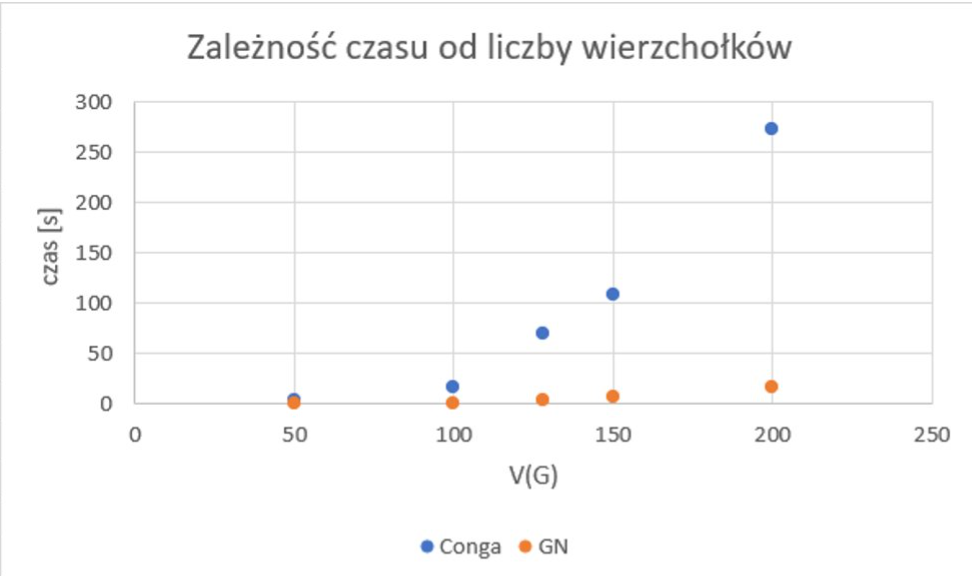
\includegraphics[width=0.7\textwidth]{images/wyk1.png}
    \caption{Zależność czasu od ilości wierzchołków}
    \label{fig:my_label}
\end{figure}

Patrząc na parametry grafów, na których czasowo uzyskiwaliśmy satysfakcjonujące wyniki postanowiliśmy znaleźć nieanonimową ligę, w której będzie występować 10 drużyn. Taką liga okazała się liga szwajcarska, a dane braliśmy od sezonu 2016/17 do sezonu 2021/22. 

\begin{figure}[H]
    \centering
    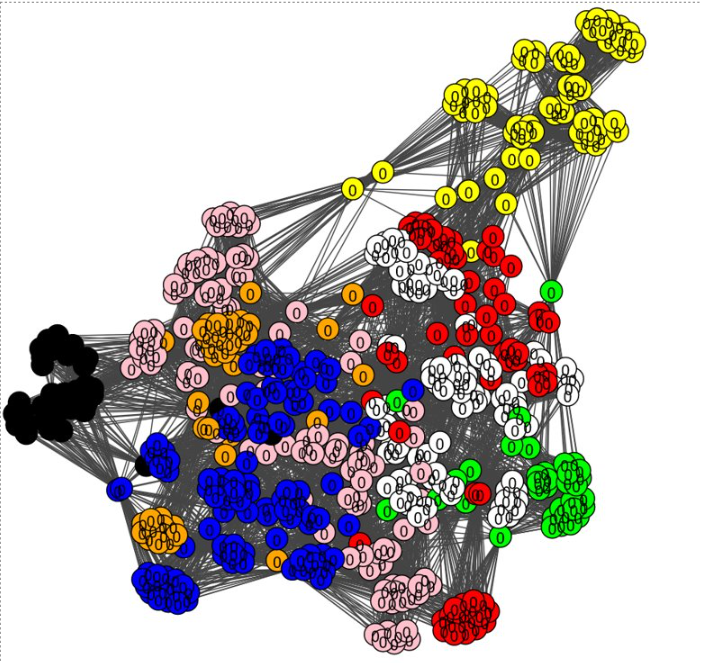
\includegraphics[width=0.7\textwidth]{images/lpa1.png}
    \caption{Wizualizacja społeczności w lidze szwajcarskiej}
    \label{fig:my_label}
\end{figure}

\subsubsection{LPA}
Algorytm LPA testowaliśmy na grafach sztucznych oraz utworzonych na podstawie prawdziwych danych wyniki prezentują się następująco

\begin{figure}[H]
    \centering
    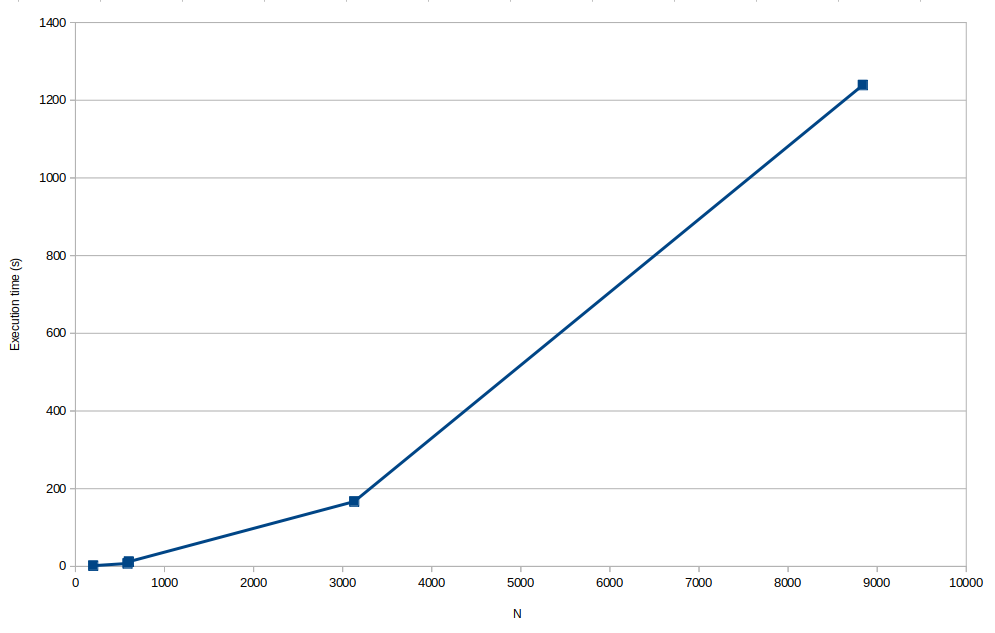
\includegraphics[width=0.7\textwidth]{images/lpa_vert.png}
    \caption{Zależność czasu od ilości wierzchołków}
    \label{fig:my_label}
\end{figure}

Czas wykonania jest podejrzanie długi, więc dodatkowo sprawdziliśmy porównanie wydajności w badaniach znalezionych w sieci.

\begin{figure}[H]
    \centering
    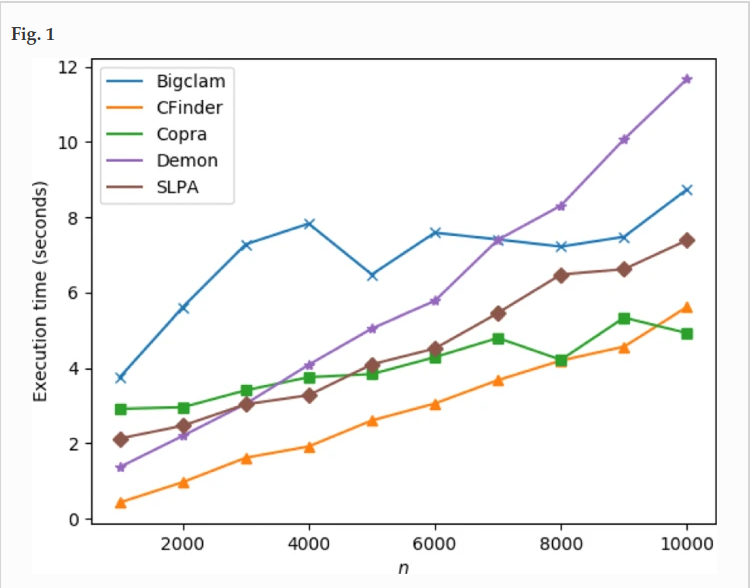
\includegraphics[width=0.7\textwidth]{images/other_vert.png}
    \caption{Zależność czasu od ilości wierzchołków dla wybranych algorytmów. 
            \href{https://appliednetsci.springeropen.com/articles/10.1007/s41109-020-00289-9}{Źródło}}
    \label{fig:my_label}
\end{figure}

\subsubsection{Nasz algorytm}
Nasz algorytm przetestowaliśmy na grafach utworzonych na bazie realnych danych. Długość wykonania zależy nie tylko od liczby wierzchołków, ale w dużym stopniu także od liczby krawędzi. Czas wykonania kształtujący się na poziomie 70 sekund dla grafu z 9 tysiącami wierzchołków jest zadowalający. Średnia złożoność czasowa jest ciężka do oszacowania. Patrząc na dane z wykresów można przypuszczać, że jest podobna do złożoności $O(nm)$.

\begin{figure}[H]
    \centering
    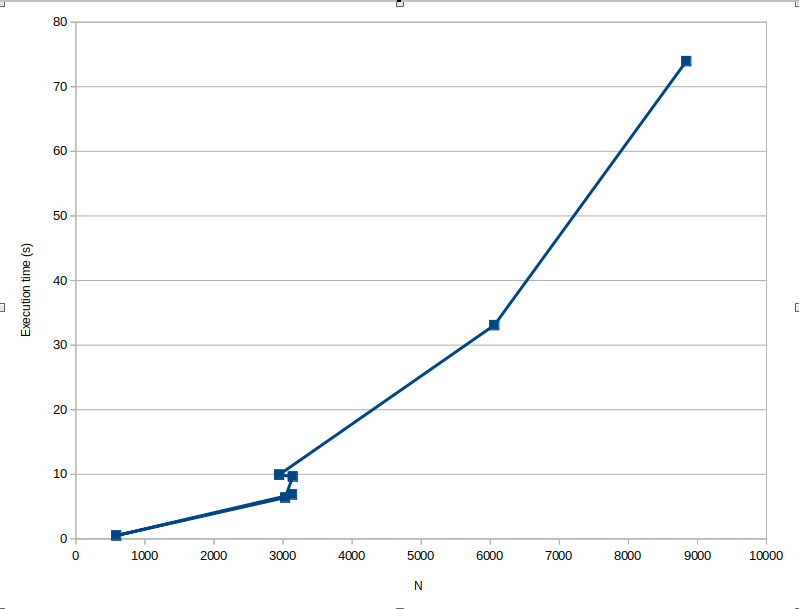
\includegraphics[width=0.7\textwidth]{images/time_vert.png}
    \caption{Zależność czasu od liczby wierzchołków}
    \label{fig:my_label}
\end{figure}

\begin{figure}[H]
    \centering
    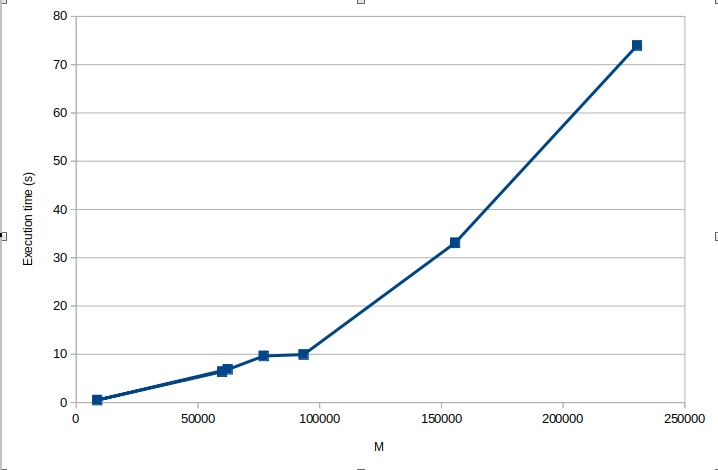
\includegraphics[width=0.7\textwidth]{images/time_edges.png}
    \caption{Zależność czasu od liczby krawędzi}
    \label{fig:my_label}
\end{figure}

\subsection{Porównanie jakości społeczności}
W społeczności piłkarskiej nie ma arbitralnego podziału na społeczności. Pierwszym etapem analizy jakościowej społeczności jest porównanie go z innym algorytmem. Wyniki porównaliśmy z algorytmem CONGA z wykorzystaniem wyznacznika Omega Index.

\subsubsection{CONGA}

Dla algorytmu CONGA testowaliśmy sztuczne grafy od 50 do 150 wierzchołków. Proces testowania polegał na wygenerowaniu grafu, obliczenia dla niego społeczności nachodzących za pomocą obu algorytmów i porównaniu według Omega Index. Eksperyment dla każdej ilości wierzchołków został powtórzony 10 razy, a następnie wyciągnęliśmy z wyników średnią.

\begin{figure}[H]
    \centering
    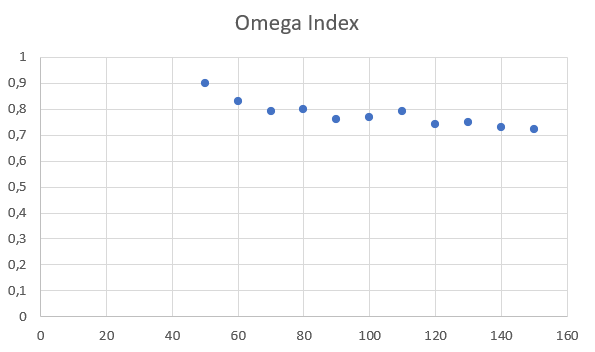
\includegraphics[width=0.7\textwidth]{images/wyk2.png}
    \caption{Porównanie społeczności otrzymanych za pomocą algorytmów CONGA i naszego}
    \label{fig:my_label}
\end{figure}

\subsubsection{LPA}

Porównywanie Omega Index algorytmu LPA z naszym dawało bardzo słabe wyniki. Niekoniecznie musiało to oznaczać, że nasz algorytm źle działa. Społeczności nie da się jednoznacznie zweryfikować i każdy algorytm będzie zwracał inne wyniki. W tym przypadku jednak algorytm LPA nie radził sobie z zadaną strukturą grafu i wyznaczał społeczności będące prawie całym grafem.

\section{Wnioski dotyczące społeczności piłkarskich}

\subsection{Analiza składu społeczności}

W momencie, gdy wiemy już, że nasz algorytm działa w zadowalającym czasie i zwraca rzeczywiste wyniki możemy wykorzystać w praktyce.

Na podstawie analizy poszczególnych społeczności, ich składu, rozmiaru i uwzględniając wiedzę piłkarską możemy zauważyć trzy różne typy społeczności zwracanych przez algorytm.

\begin{enumerate}
    \item Małe społeczności, mniej niż 10 piłkarzy z reguły są to zawodnicy związani ze sobą przez parę sezonów, którzy nie mają na swoim koncie dużo klubów, ale znalazły się przypadki odbiegające od tego schematu
    \item Średnie społeczności, 10-25 piłkarzy, są to piłkarze, którzy reprezentowali jeden klub przez okres około 2-3 sezonów
    \item Duże społeczności, ok 30. piłkarzy, są to albo piłkarze połączeni z kilku klubów, którzy dzięki transferom na przestrzeni kilku lat wytworzyli pomiędzy sobą relacje lub piłkarze, którzy reprezentowali jeden klub przez długi (ok. 10 lat) okres czasu jeden klub, ale niekoniecznie w tym samym czasie
\end{enumerate}

Prezentacje przykładów społeczności podanych powyżej zaprezentujemy na podstawie ligi angielskiej:

Ad 1. Podamy dwa przykłady. Pierwszym będzie pięciu piłkarzy Manchesteru City: 

\begin{figure}[H]
    \centering
    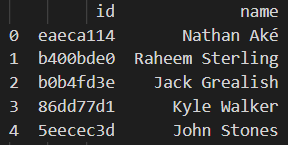
\includegraphics[width=0.5\textwidth]{images/city.png}
    \caption{Pięciu piłkarzy Man City}
    \label{fig:my_label}
\end{figure}

Kyle Walker, John Stones oraz Raheam Sterling grają już dobre parę lat razem w klubie i poza nim reprezentowali tylko jeden inny klub, do tego dołączają Jack Grealish oraz Nathan Ake, którzy występują w Manchesterze od niedawna.

Drugi przykład dotyczy pięciu graczy, z których żadnych 3 nie grało na raz razem w jednym klubie.

\begin{figure}[H]
    \centering
    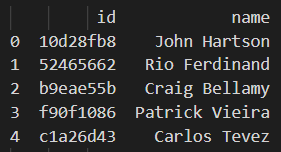
\includegraphics[width=0.5\textwidth]{images/vieira.png}
    \caption{Piłkarze różnych klubów}
    \label{fig:my_label}
\end{figure}

Jest to ciekawy przykład pokazujący tworzenie się mini społeczności pomiędzy klubami.

Ad 2. Zaprezentujemy przykład łączący piłkarzy Chelsea i Arsenalu:

\begin{figure}[H]
    \centering
    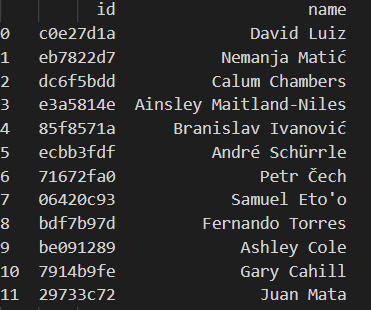
\includegraphics[width=0.5\textwidth]{images/chearse.png}
    \caption{Piłkarze Chelsea i Arsenalu}
    \label{fig:my_label}
\end{figure}

Ta społeczność składa się głównie z piłkarzy Chelsea na przestrzeni lat 2006-2019. Do tej społeczności należą również gracze, którzy nie reprezentowali Chelsea tylko Arsenal, mianowicie Calum Chambers oraz Ainsley Maitland-Niles. Stało się tak ponieważ Petr Cech i David Luiz odpowiednio w 2015 i 2019 roku zmienili swoje barwy klubowe z Chelsea na Arsenal co poskutkowało wytworzeniem się relacji z piłkarzami Arsenalu.
Jest to ciekawy przykład, któy możemy rozpatrywać w kontekście utworzenia optymalnej drużyny pod względem zgrania.

Ad 3. Zaprezentujemy przykład wielu piłkarzy reprezentujący jeden klub na przestrzeni wielu lat

\begin{figure}[H]
    \centering
    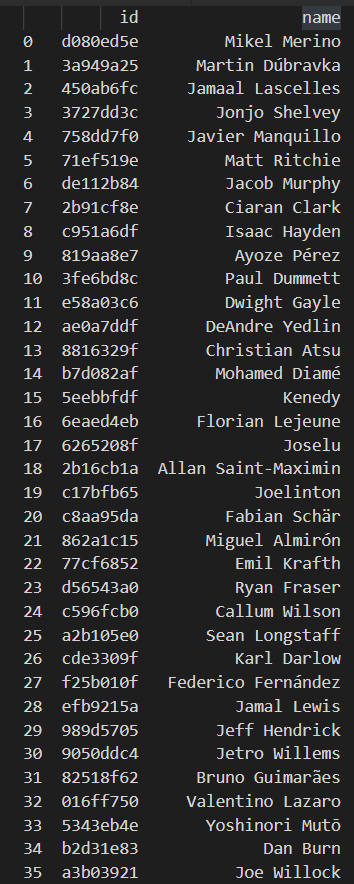
\includegraphics[width=0.5\textwidth]{images/newcastle.png}
    \caption{Piłkarze Newcastle}
    \label{fig:my_label}
\end{figure}

Widzimy w przykładzie graczy Newcastle United na przestrzeni lat 2014-2022. Średnia czasu gry jednego piłkarza w tym klubie wynosiła ok. 4 lata.

\subsection{Analiza ilości i wielkości społeczności}

Przepuściliśmy nasz algorytm przez siedem grafów: pięć najlepszych lig z osobna, pięć lig skonwertowanych w jeden graf i przez polską Ekstraklasę. Dla każdego grafu zaprezentujemy ilość wierzchołków, ilość krawędzi, ilość wyznaczonych społeczności oraz histogram społeczności.

\begin{figure}[H]
    \centering
    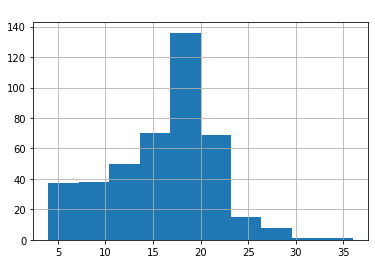
\includegraphics[width=0.5\textwidth]{images/hpl.png}
    \caption{Premier League 3130 wierzchołków 62234 krawędzi  425 społeczności}
    \label{fig:my_label}
\end{figure}

\begin{figure}[H]
    \centering
    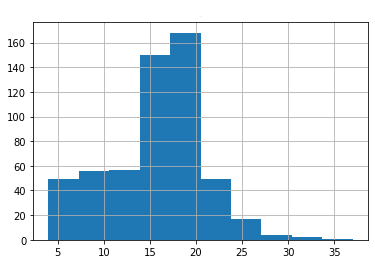
\includegraphics[width=0.5\textwidth]{images/hla.png}
    \caption{La liga 3701 wierzchołków 79409 krawędzi 553 społeczności}
    \label{fig:my_label}
\end{figure}

\begin{figure}[H]
    \centering
    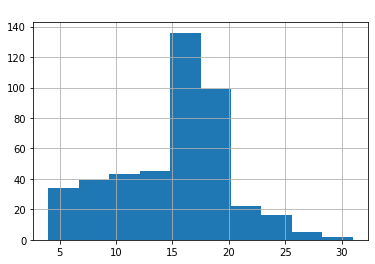
\includegraphics[width=0.5\textwidth]{images/hbu.png}
    \caption{Bundesliga 3030 wierzchołków 59932 krawędzi 441 społeczności}
    \label{fig:my_label}
\end{figure}

\begin{figure}[H]
    \centering
    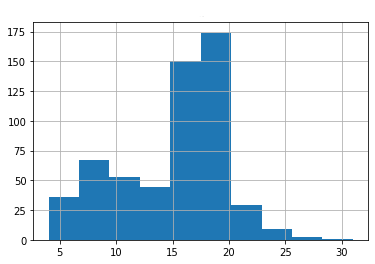
\includegraphics[width=0.5\textwidth]{images/hsa.png}
    \caption{Serie A 3141 wierzchołków 77026 krawędzi 565 społeczności}
    \label{fig:my_label}
\end{figure}

\begin{figure}[H]
    \centering
    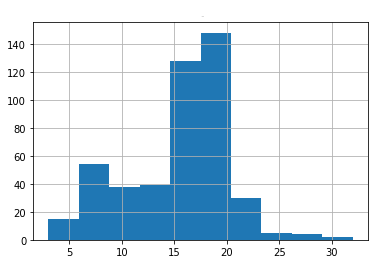
\includegraphics[width=0.5\textwidth]{images/hl1.png}
    \caption{Ligue 1 3063 wierzchołków 63745 krawędzi 463 społeczności}
    \label{fig:my_label}
\end{figure}

\begin{figure}[H]
    \centering
    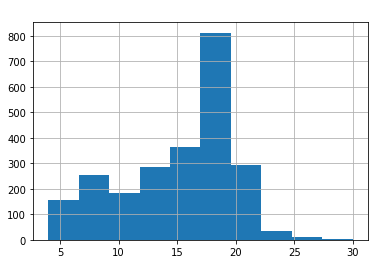
\includegraphics[width=0.5\textwidth]{images/histtop5.png}
    \caption{Top 5 16065 wierzchołków 342346 krawędzi 2393 społeczności}
    \label{fig:my_label}
\end{figure}

\begin{figure}[H]
    \centering
    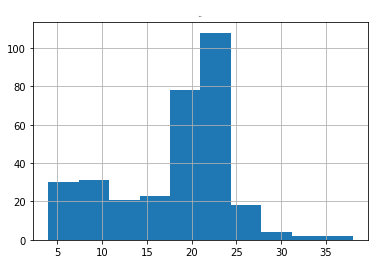
\includegraphics[width=0.5\textwidth]{images/heks.png}
    \caption{Ekstraklasa 2398 wierzchołków 60473 krawędzi 317 społeczności}
    \label{fig:my_label}
\end{figure}

Jak widać powyżej histogramy przyjmują podobne kształty dla każdego z rozważanych grafów. Świadczy to o podobnej strukturze każdego z grafów i o tym że każda liga nie wyróżnia się z pozostałych na tle wewnętrznych transferów pomiędzy nimi.

\subsection{Wnioski}
Po szczegółowej analizie każdego z grafów i społeczności zwracanych przez nasz algorytm dochodzimy do następujących wniosków:

\begin{itemize}
    \item Algorytm dobrze działałby w kontekście zwrócenia drużyny złożonej z najczęściej występujących w niej piłkarzy na przestrzeni kilku lat. Można to nazywać ikonicznym składem pięcio/dziesięciolecia.
    \item Algorytm słabo działa w kontekście szukania powiązań pomiędzy drużynami. Znalezienie średniej społeczności jak z przykładu z podpunktu 7.1 jest bardzo trudne. Możliwe, że przy implementacji dodatkowych narzędzi można to ułatwić
    \item Nie widać przesłanek na temat trendów transferowych pomiędzy drużynami wewnątrz ligi i pomiędzy ligami w ligach top5. Możliwe, że brak uwzględniania wszystkich lig europejskich jest czynnikiem, który to uniemożliwia. Jednak po uwzględnieniu ich wynikowy graf mógłby okazać się zbyt duży.
\end{itemize}

Proponowane modyfikacje na przyszłość:

\begin{itemize}
    \item Sklejanie społeczności, kiedy mają wystarczająco dużo wspólnych piłkarzy.
    \item Zmodyfikowanie algorytmu, żeby działał na grafie ważonym, gdzie wagi to ilość meczów rozegranych pomiędzy zawodnikami. Potem można byłoby modyfikować graf poprzez usuwanie krawędzi o mniejszych niż podana minimalna liczba meczów. Mogłoby to rozwiązać problem optymalnej drużyny.
\end{itemize}

\section{Podsumowanie}

Podsumowując, udało się zaimplementować nasz własny algorytm i porównać go z istniejącym rozwiązaniem problemu. Nasz algorytm działa w zadowalającym nas czasie. Udało nam się dobrze dopasować dane do eksperymentów. Algorytm dobrze rozpoznaje drużyny piłkarskie i dopasowuje do nich zawodników.

Z drugiej jednak strony nie wszystko udało nam się zweryfikować. W zwracanych społecznościach ciężko znaleźć społeczności, które rozwiązywałyby problem optymalnej drużyny. Wymaga to dużej wiedzy eksperckiej lub zaimplementowania dodatkowych narzędzi do identyfikacji piłkarzy. Przy aktualnej implementacji algorytmu nie możemy wyciągnąć wniosków na temat trendów transferowych.


\section{Bibliografia}

\begin{enumerate}

    \item Overlapping community detection at scale: a nonnegative matrix factorization approach - Jaewon Yang, Jure Leskovec
    \item A comparative study of overlapping
community detection methods from the
perspective of the structural properties - Vinícius da Fonseca Vieira , Carolina Ribeiro Xavier, Alexandre Gonçalves Evsukoff
    \item Omega Index of Line and Total Graphs - Musa Demirci , Sadik Delen , Ahmet Sinan Cevik , and Ismail Naci Cangul
    \item www.fbref.com
\end{enumerate}

\end{document}
